\documentclass[AutoFakeBold,AutoFakeSlant]{beamer}

\usepackage[british]{babel}
\usepackage{graphicx,hyperref,sysu,url}

%% 中文
\usepackage{ctex}

%\usepackage{newtxmath}
\RequirePackage{booktabs}
\usepackage{multicol} 
\usepackage{multirow}
\usepackage[ruled,linesnumbered]{algorithm2e}
\usepackage{color}

% 数学公式
\usepackage{amsmath,bm}
\usepackage{lmodern}
\usepackage{utopia} %font utopia imported
\usepackage{amsfonts}
\usepackage{amsthm}
\usepackage{amssymb}

% colors
\definecolor{sysugreen}{RGB}{0,88,38}
\definecolor{sysugreendark}{RGB}{5,71,25}

% commands
\newcommand{\ctoday}{\number\year 年 \number\month 月 \number\day 日}

%% 根据需要修改中文字体
\setCJKmainfont[ItalicFont={SimSun}]{SimSun}
% \setCJKsansfont{Microsoft YaHei}
\setCJKsansfont{SimHei}
\setCJKmonofont{FangSong}

% \setCJKmonofont{SimSun}
% \xeCJKsetcharclass{"0}{"2E7F}{0}
% \xeCJKsetcharclass{"2E80}{"FFFF}{1}

% Require XeLaTeX
\RequirePackage{fontspec,xltxtra,xunicode}
% 根据需要修改英文字体
\setmainfont[Mapping=tex-text]{Times New Roman}
\setsansfont[Mapping=tex-text]{Arial}
\setmonofont{Consolas}

% 设置公式字体
\usefonttheme[onlymath]{serif}

% 参考文献样式
\bibliographystyle{IEEETran}


% 演示文稿标题:
%  1 底部显示的标题;
%  2 标题页正中显示的大标题;
\title[多模态大模型项目开题报告]{基于强化学习决策的文档理解与检索多模态问答系统}

% 可选：标题页显示的副标题
%\subtitle{副标题}

% 作者信息:
%  1 底部显示的作者信息;
%  2 联系信息;
% \author[Author Name]{
%   答辩人 \\\medskip
%   {\small \url{netid@mail2.sysu.edu.cn}} \\
%   {\small \url{www.sysu.edu.cn}}
% }

% 学校学院信息:
%  1 顶部学校信息
%  2 标题页显示的学院学校信息
\institute[Sun Yat-Sen University]{
  中山大学计算机学院
  }

%% 时间信息
%  1 底部显示的标准时间信息
%  2 标题页显示的中文时间信息
\date[\today]{\ctoday}


\begin{document}
\newtheorem{assumption}{假设}

% 作者信息
\author[刘天翔\quad 杨毅涵\quad  郭翊涛]{
  刘天翔\quad 杨毅涵\quad  郭翊涛 
  \texorpdfstring{\\\medskip {\small 计算机科学与技术}}{}
}

\begin{frame}
  % 标题页
  \titlepage
\end{frame}
% 标题页不编号
\setcounter{framenumber}{0}

\begin{frame}
  % 目录页
  \frametitle{目\quad 录}
  % 双栏
  % \begin{multicols}{2}
  %   \tableofcontents
  % \end{multicols}
  \tableofcontents[hideallsubsections]
\end{frame}

\section{研究背景与目标}

\begin{frame}
  \frametitle{研究背景}
  \begin{itemize}
    \item 在学习和生活中关键信息分布在 PDF、PPT、扫描件等非结构化文档
    \item 传统的RAG 主要针对纯文本数据设计，忽略了文档中丰富的视觉结构信息
    \item 随着多模态大语言模型（MLLM）的快速发展，模型能够直接处理视觉输入的能力，使得多模态 RAG 成为提升文档理解效率的关键技术路径
  \end{itemize}
\end{frame}

\begin{frame}
  \frametitle{任务定义与核心目标}
  \begin{itemize}
    \item 构建可自主决策的多模态文档智能助手，在生成回答的同时，精准定位并标注引用的页面坐标、图表编号或视频时间戳
    \item 多模态RAG 架构构建：建立统一的向量索引池，将文本语义、表格结构描述与图像/视频的视觉特征进行跨模态对
    \item 通过 GRPO 强化学习训练轻量路由模型，选择合适 VLM 推理
  \end{itemize}
\end{frame}

\section{相关工作调研}

\begin{frame}
  \frametitle{相关工作调研（1）}
  \begin{itemize}
    \item \textit{RAG-Anything: All-in-One RAG Framework} \cite{guo2025raganythingallinoneragframework}
    
    该框架构建了覆盖 PDF 与图像等文件的全模态解析流水线
    \item \textit{Scaling Beyond Context: A Survey of Multimodal RAG for Document Understanding} \cite{gao2025scaling}
    
    该综述探讨了多模态 RAG 克服传统 OCR 提取局限的技术路径，强调通过视觉模型直接理解图表与排版

    \item \textit{ColPali: Efficient Document Retrieval with Vision Language Models} \cite{faysse2024colpali}
    
    ColPali 摒弃繁琐 OCR 预处理的端到端视觉空间检索架构，而是直接将视觉语言模型直接应用于文档图像嵌入
  \end{itemize}
\end{frame}

\begin{frame}
  \frametitle{相关工作调研（2）}
  \begin{itemize}
    \item \textit{DeepSeek-OCR 2: Visual Causal Flow} \cite{wei2026deepseekocr2visualcausal}
    
    DeepSeek-OCR-2 能直接将多页复杂文档转化为包含排版与定位框标记等视觉结构信息的 Markdown 文件

    \item \textit{Efficient Motion-Aware Video MLLM} \cite{zhao2025efficientmotionawarevideomllm}
    
    该研究设计了一种能够高效处理动态视频序列的运动感知多模态大模型

    \item RAGFlow （\url{https://github.com/infiniflow/ragflow}）
    
    项目RAGFlow 是一款为处理复杂排版数据而构建的开源 RAG 框架
  \end{itemize}
\end{frame}

\section{系统架构}

\begin{frame}
  \frametitle{系统架构图}
  \begin{figure}[htbp]
    \centering
    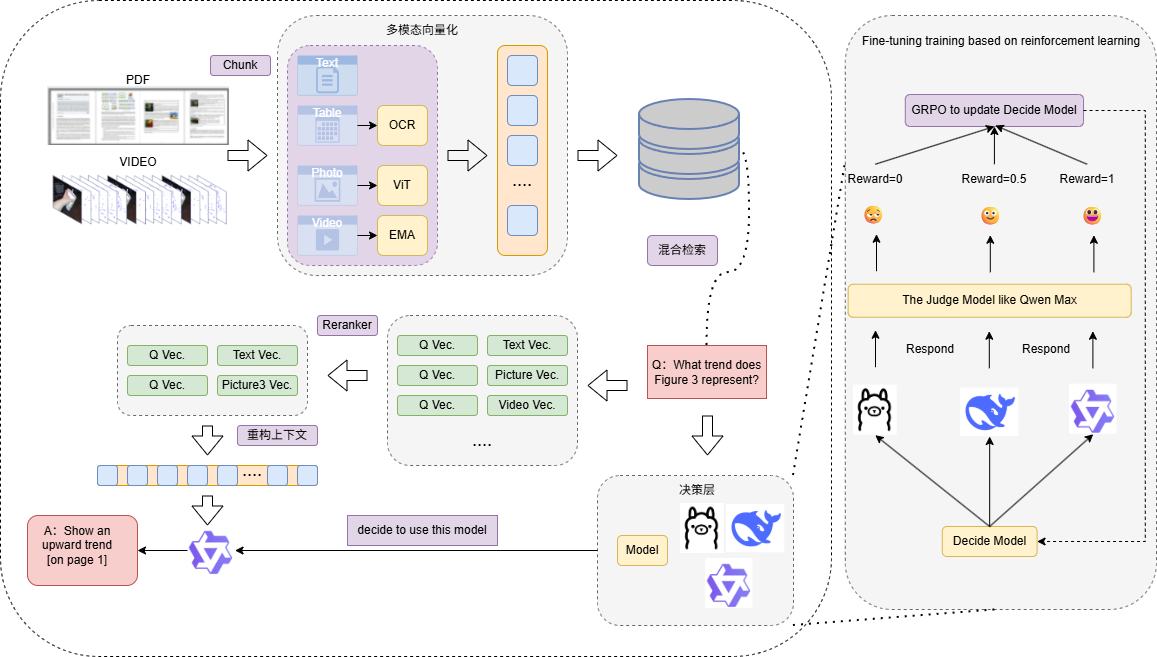
\includegraphics[width=0.92\textwidth]{image/frame.png}
  \end{figure}
\end{frame}

\begin{frame}
  \frametitle{模型路由决策模块}
  \begin{itemize}
    \item 基于意图分类的前置决策层，选择最优多模态模型路径
    \item 训练阶段生成多种决策，由评测模型给分
    \item 使用 GRPO 更新路由权重，使其在不同问题类型上自适应选择
  \end{itemize}
\end{frame}

\begin{frame}
  \frametitle{多模态向量化}
  \begin{itemize}
    \item 文本：BGE-m3 向量化形成基础索引
    \item 表格：OCR 转 Markdown，保留结构化特征后向量化
    \item 图片：ViT 等视觉编码提取特征并保留空间位置信息
    \item 视频：运动感知 MLLM 融合时序特征，降低冗余 token
  \end{itemize}
\end{frame}

\begin{frame}
  \frametitle{在线检索与决策}
  \begin{itemize}
    \item 混合检索：同时检索文本库、表格 Markdown 与视觉摘要
    \item Rerank 重排序：BGE-Reranker-v2-m3 二次打分，过滤噪声
  \end{itemize}
\end{frame}

\begin{frame}
  \frametitle{Generation 生成阶段}
  \begin{itemize}
    \item 上下文构建：拼接文本、表格与视觉描述，形成结构化输入
    \item VLM 推理：通过 prompt 约束标注页码、图表来源等溯源信息
  \end{itemize}
\end{frame}

\section{模型与评测}

\begin{frame}
  \frametitle{模型选择}
  \begin{itemize}
    \item Decide 决策模型：Qwen-0.5B + GRPO 强化学习
    \item 嵌入模型：DeepSeek-OCR-2，BGE-Reranker-v2-m3
    \item VLM：Qwen2.5-VL，LLaMA 3.2 Vision，DeepSeek-VL
  \end{itemize}
\end{frame}

\begin{frame}
  \frametitle{评测数据集与指标}
  算力预算
  \begin{itemize}
    \item NVIDIA GeForce RTX 5090 32GB $\times$ 1
    \item NVIDIA GeForce RTX 3070  8GB $\times$ 1
  \end{itemize}

  评测数据集与指标
  \begin{itemize}
    \item 数据集：DocVQA、ChartQA 子集（必要时自建数据集）
    \item 检索与路由：Recall@K、MRR
    \item 回答质量：ANLS、EM
  \end{itemize}
\end{frame}

\section{计划与预期}

\begin{frame}
  \frametitle{时间计划与预期成果}
  \resizebox{0.95\textwidth}{!}{%
  \begin{tabular}{|l|c|c|c|}
      \hline
      时间 & 任务 & 具体内容 & 完成情况 \\
      \hline
      2026.3.5--2026.4.15(6weeks) & 确定选题、文献调研 & 确定小组项目选题，并完成相关论文和项目调研 & $\checkmark$ \\
      \hline
      2026.4.16--2026.5.7(4weeks) & 系统设计、开题报告 & 完成系统架构与开题报告材料撰写 & $\checkmark$ \\
      \hline
      2026.5.7 & 制作PPT、上台展示 & 完成开题报告展示材料与答辩 & $\checkmark$ \\
      \hline
      2026.5.8--2026.6.11(4weeks) & 项目开发与实现 & 任务分工并开发核心功能 & \\
      \hline
      2026.6.12--2026.6.17(1week) & 项目评测 & 验证基础功能并完成评测 & \\
      \hline
      2026.6.18--ddl & 最终报告的撰写 & 完成最终项目报告 & \\
      \hline
      ddl & 期末验收 & 准备期末展示材料：PPT、demo等 & \\
      \hline
  \end{tabular}%
  }
  \\
  预期成果
  \begin{itemize}
    \item 文档智能助手系统原型，支持检索问答与引用溯源
    \item 代码实现与技术文档（训练、集成、部署与测试说明）
    \item 完整项目报告，包含实验结果、可视化与反思展望
    \item 期末验收：PPT 与 Demo 用于期末验收
  \end{itemize}

\end{frame}

\section*{致谢}
\section*{参考文献}
\begin{frame}[allowframebreaks]
  \frametitle{参考文献}
  \bibliography{../../Proposal/sysu-thesis/reference}
\end{frame}

\begin{frame}
  \frametitle{谢谢}
  感谢老师与同学们的聆听。
\end{frame}
\end{document}
